% !TEX root=../document.tex

\section{Conceptual model}

\subsection{System sequence diagrams}

\subsubsection{SSD - Configure Message Format}
\begin{figure}[!htbp]
  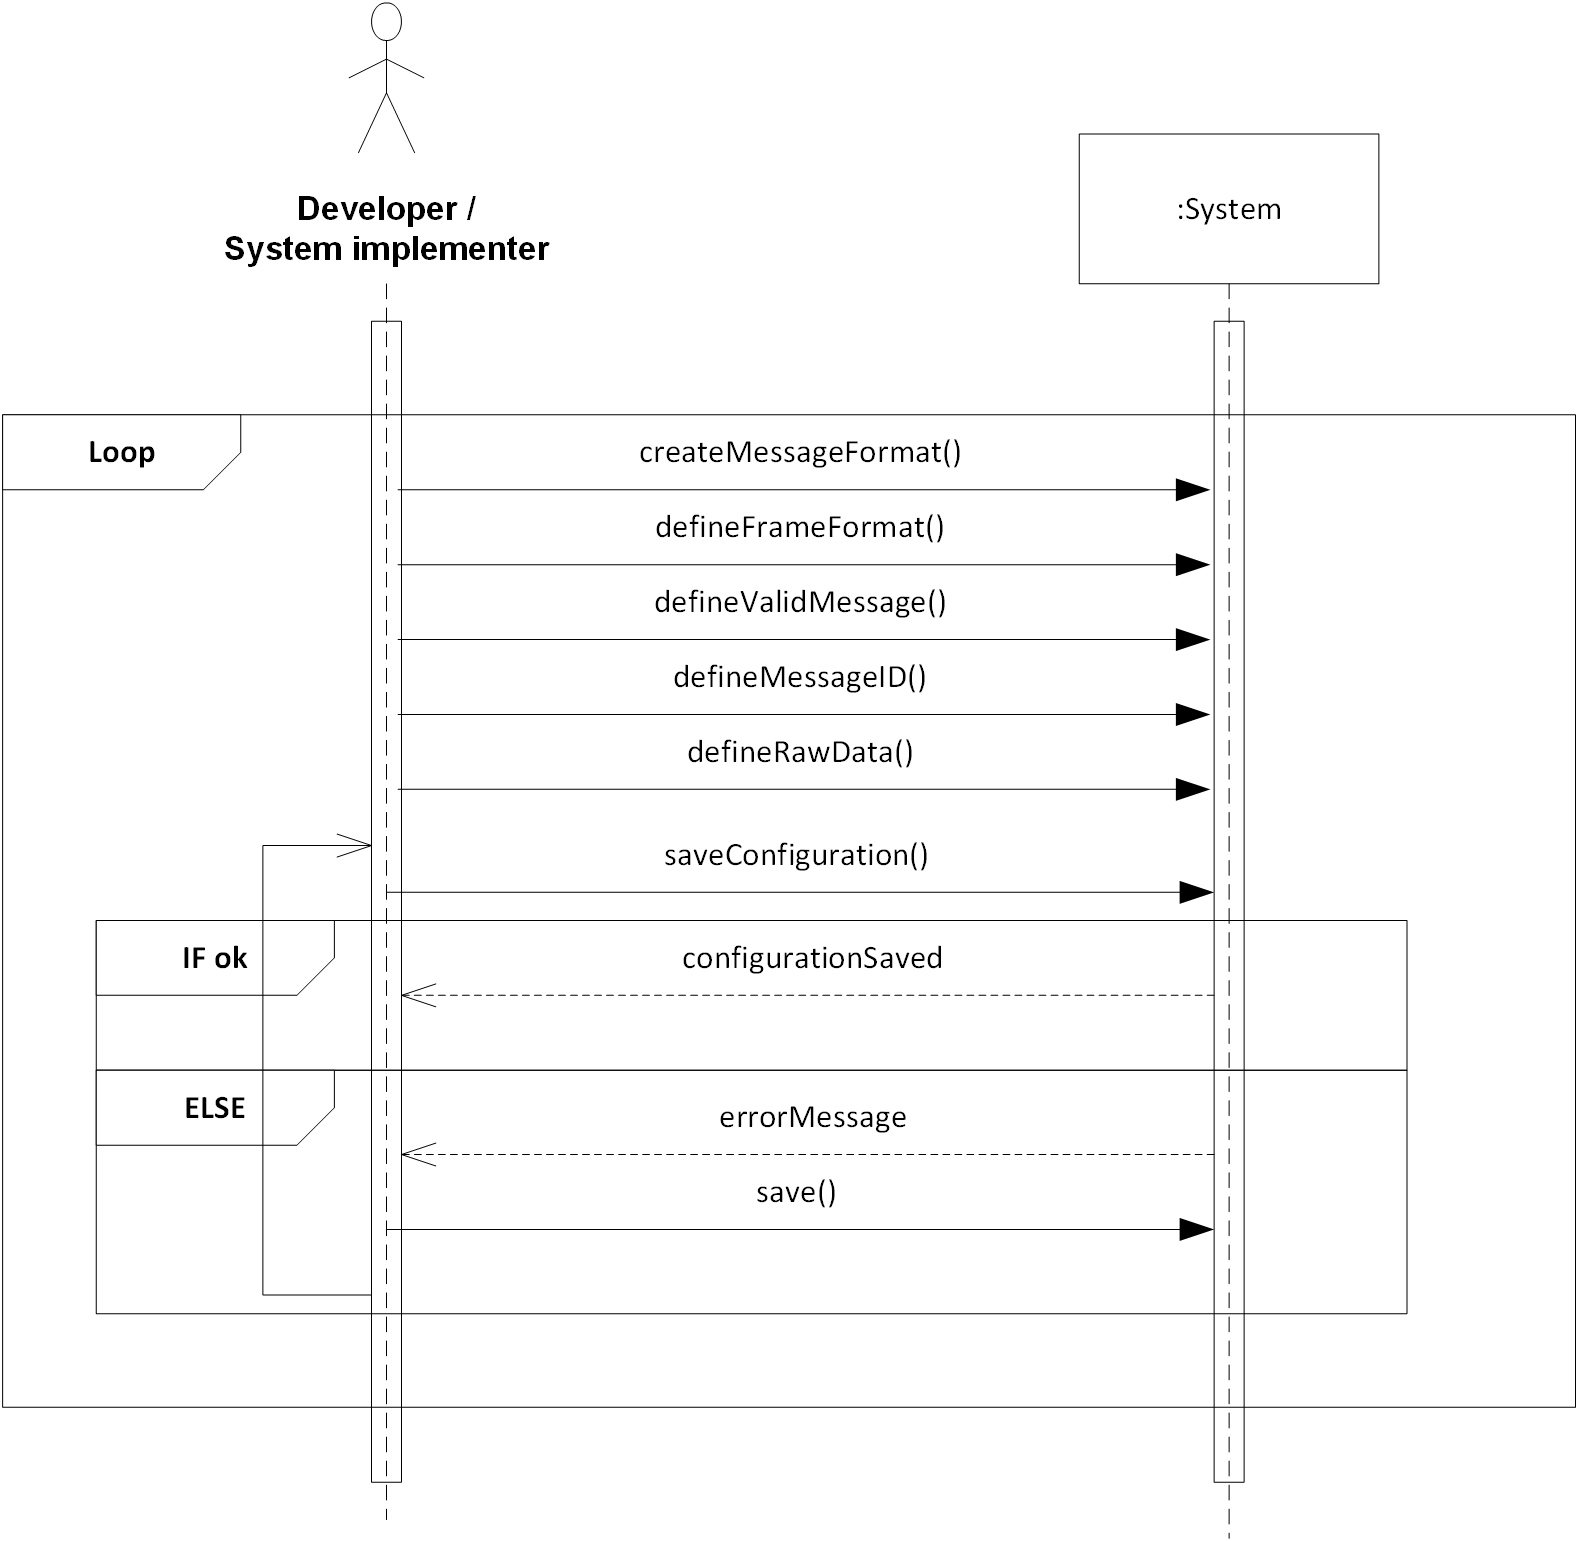
\includegraphics[width=\textwidth]{SSD-Configure-Message-Format.png}
  \caption{SSD for UC\vref{uc_formatconf}}
  \label{fig:SSD-Configure-Message-Format}
\end{figure}
\clearpage

\subsubsection{SSD - Configure Sensors}
\begin{figure}[!htbp]
  \ContinuedFloat
  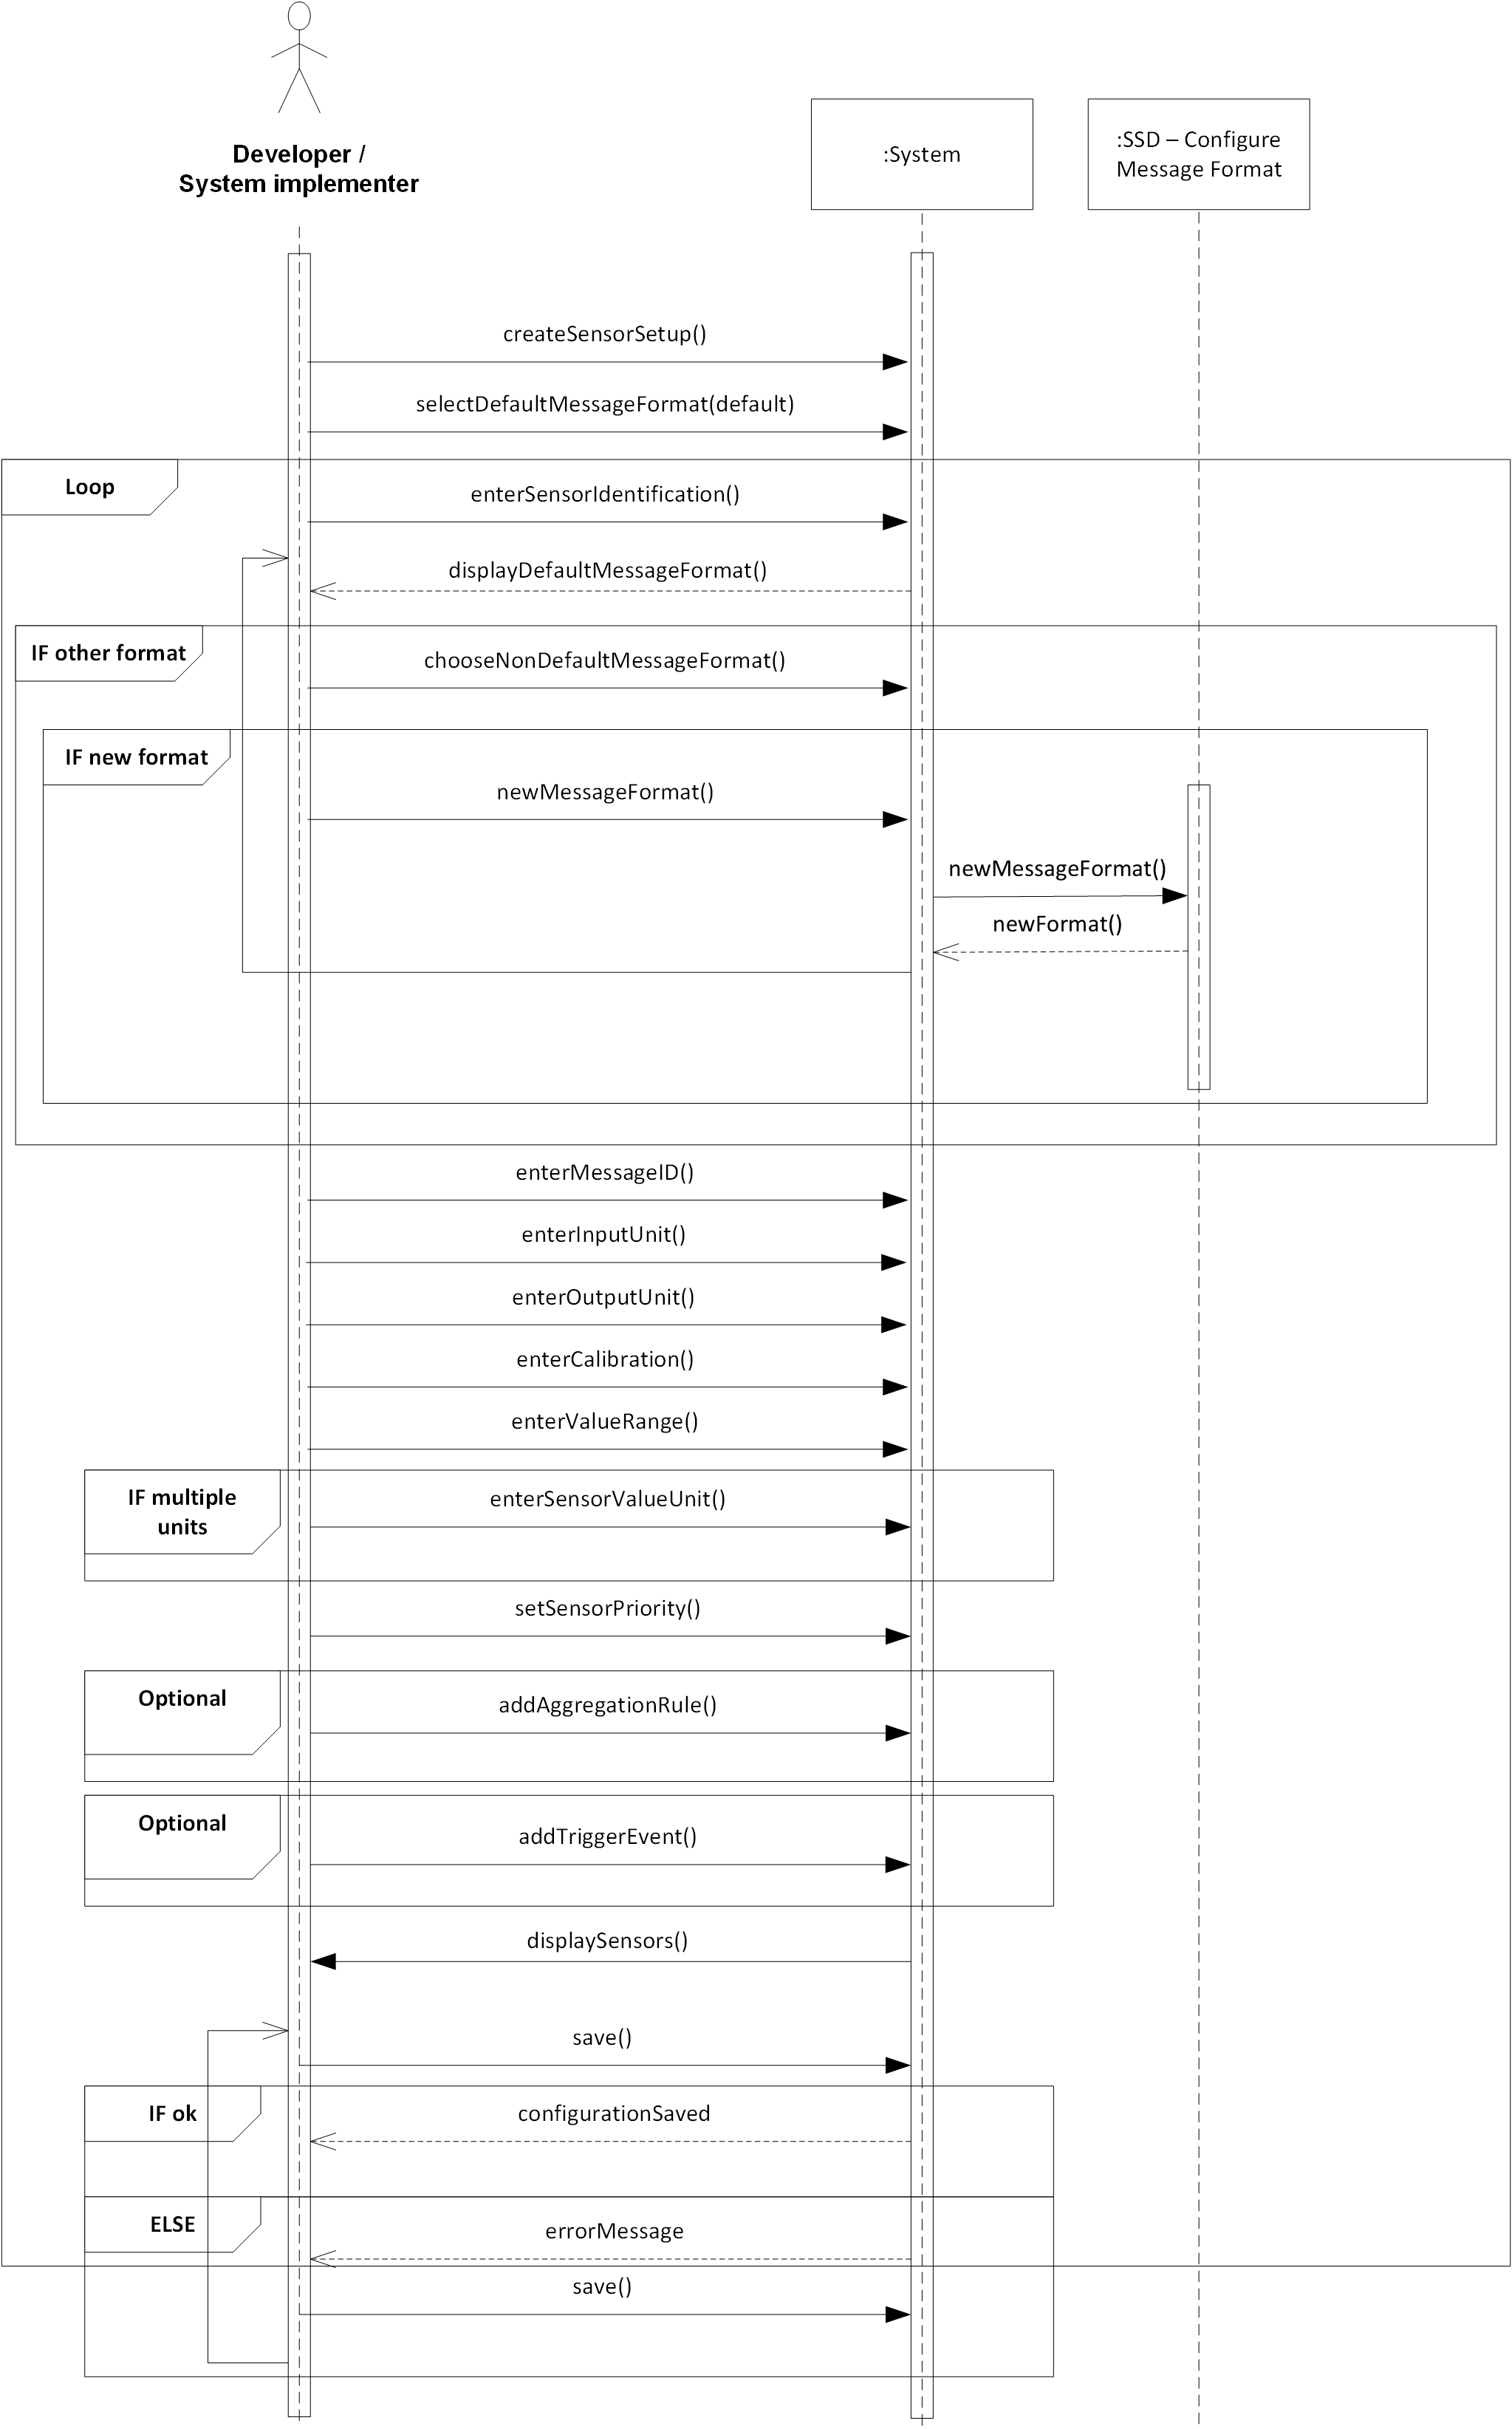
\includegraphics[height=0.9\textheight]{SSD-Configure-Sensors.png}
  \caption{SSD for UC\vref{uc_sensconf}}
  \label{fig:SSD-Configure-Sensors}
\end{figure}
\clearpage

\subsubsection{SSD - Configure Display}
\begin{figure}[!htbp]
  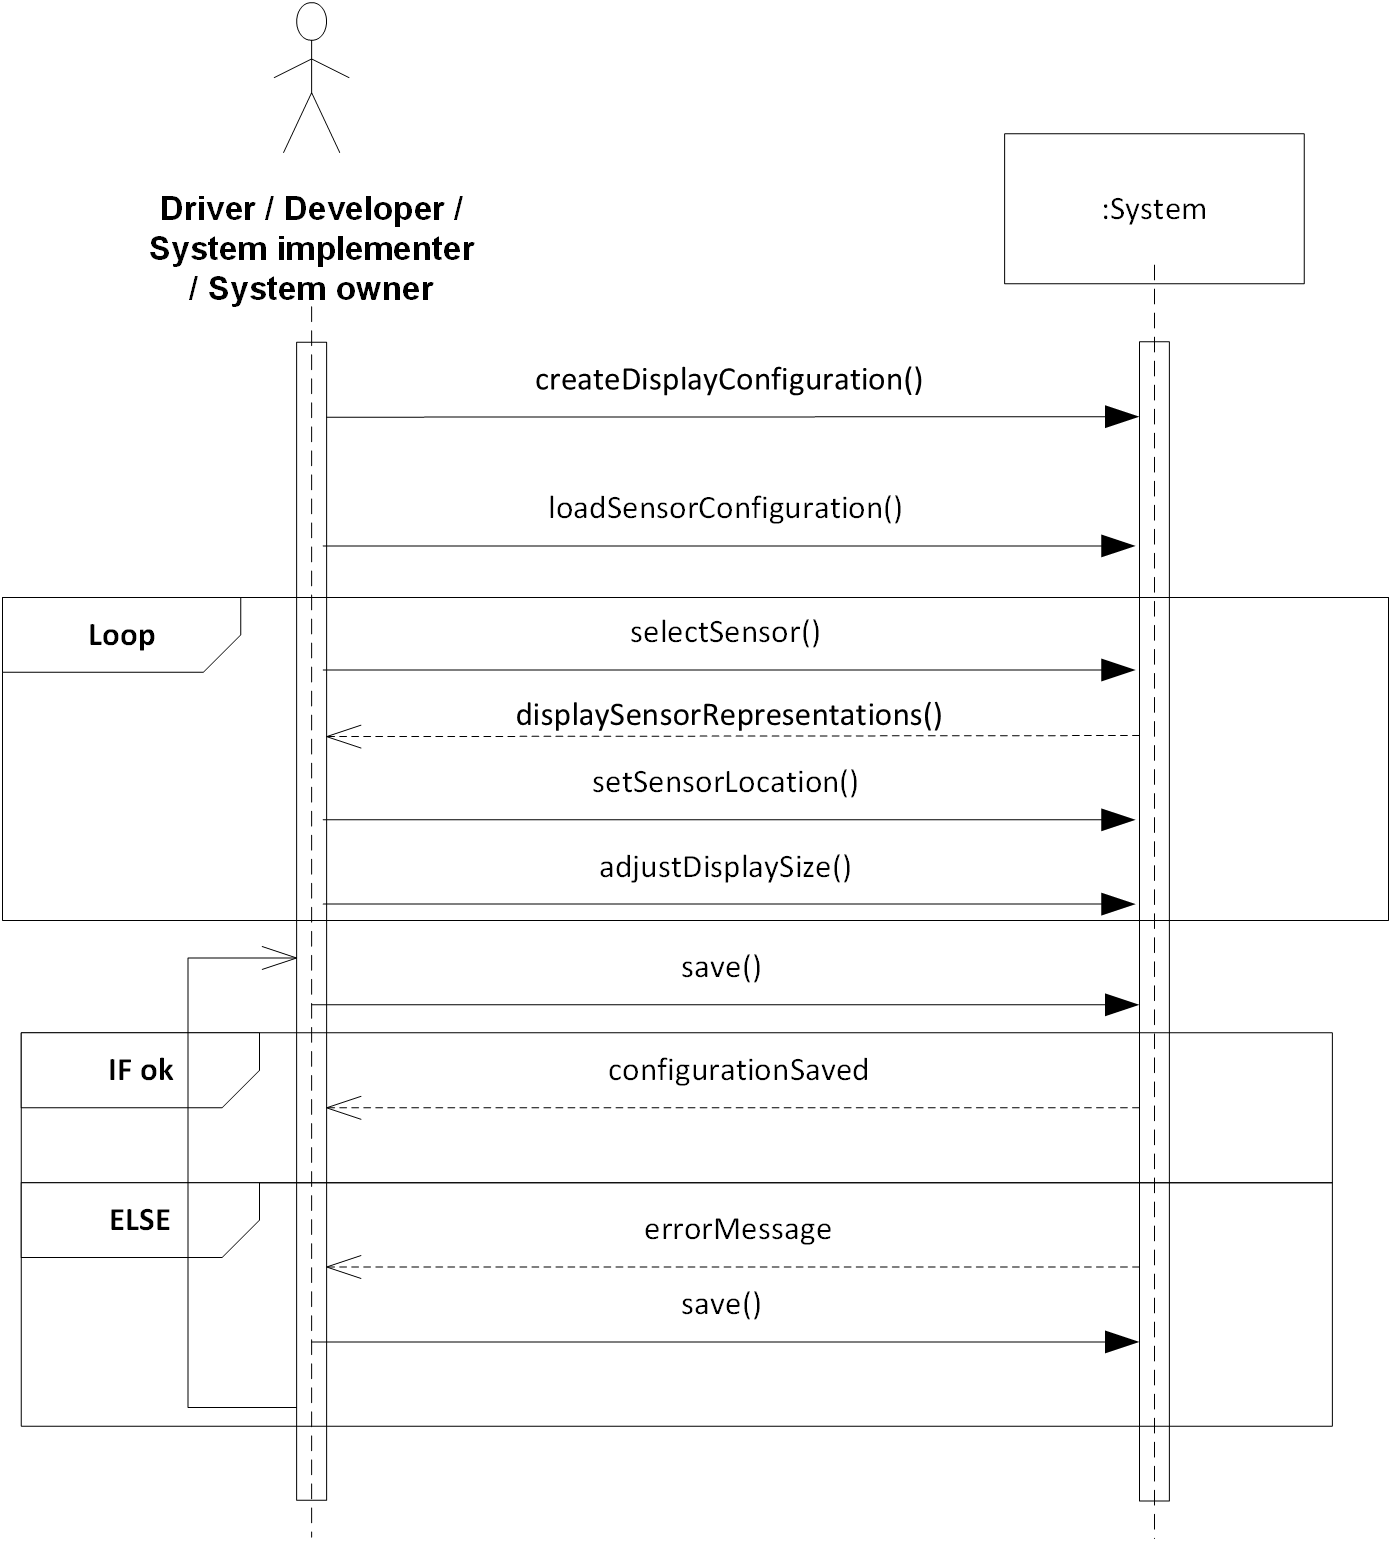
\includegraphics[width=\textwidth]{SSD-Configure-Display.png}
  \caption{SSD for UC\vref{uc_dispconf}}
  \label{fig:SSD-Configure-Display}
\end{figure}
\clearpage 


\subsubsection{SSD - Upload Configuration}
\begin{figure}[!htbp]
  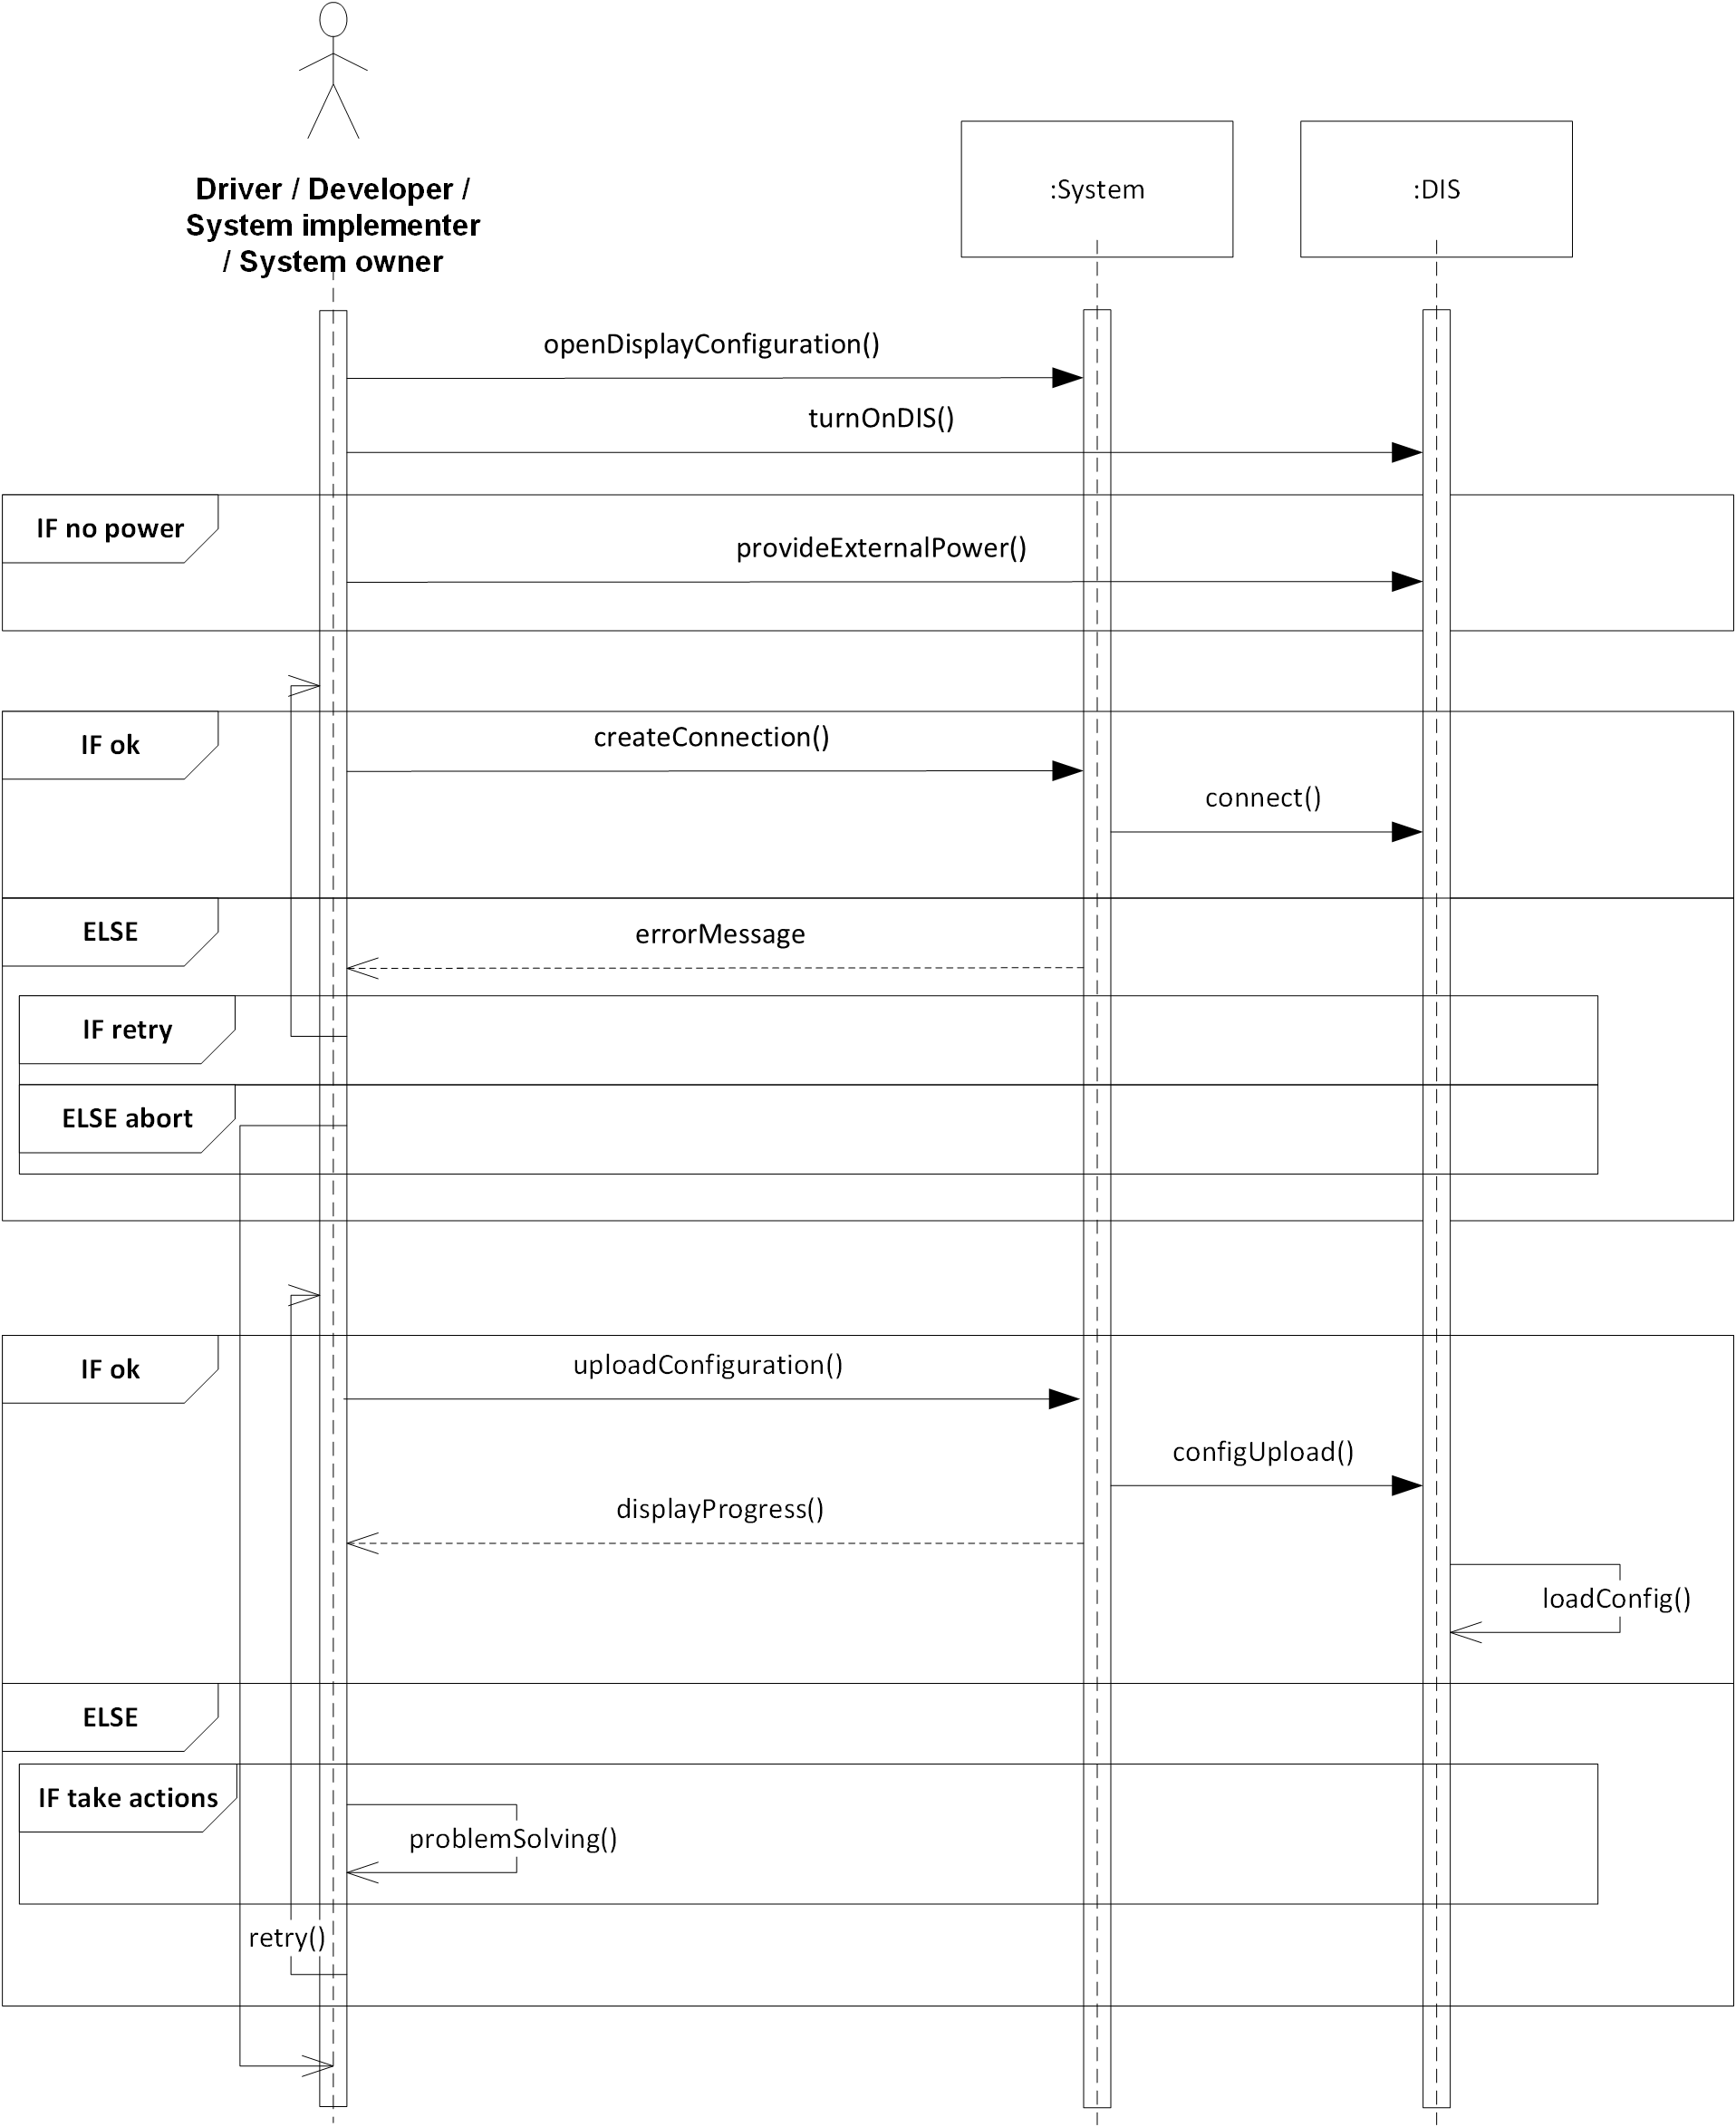
\includegraphics[width=\textwidth]{SSD-Upload-Configuration.png}
  \caption{SSD for UC\vref{uc_dispconf}}
  \label{fig:SSD-Upload-Configuration}
\end{figure}
\clearpage 


\subsubsection{SSD - Send message to driver}
\begin{figure}[!htbp]
  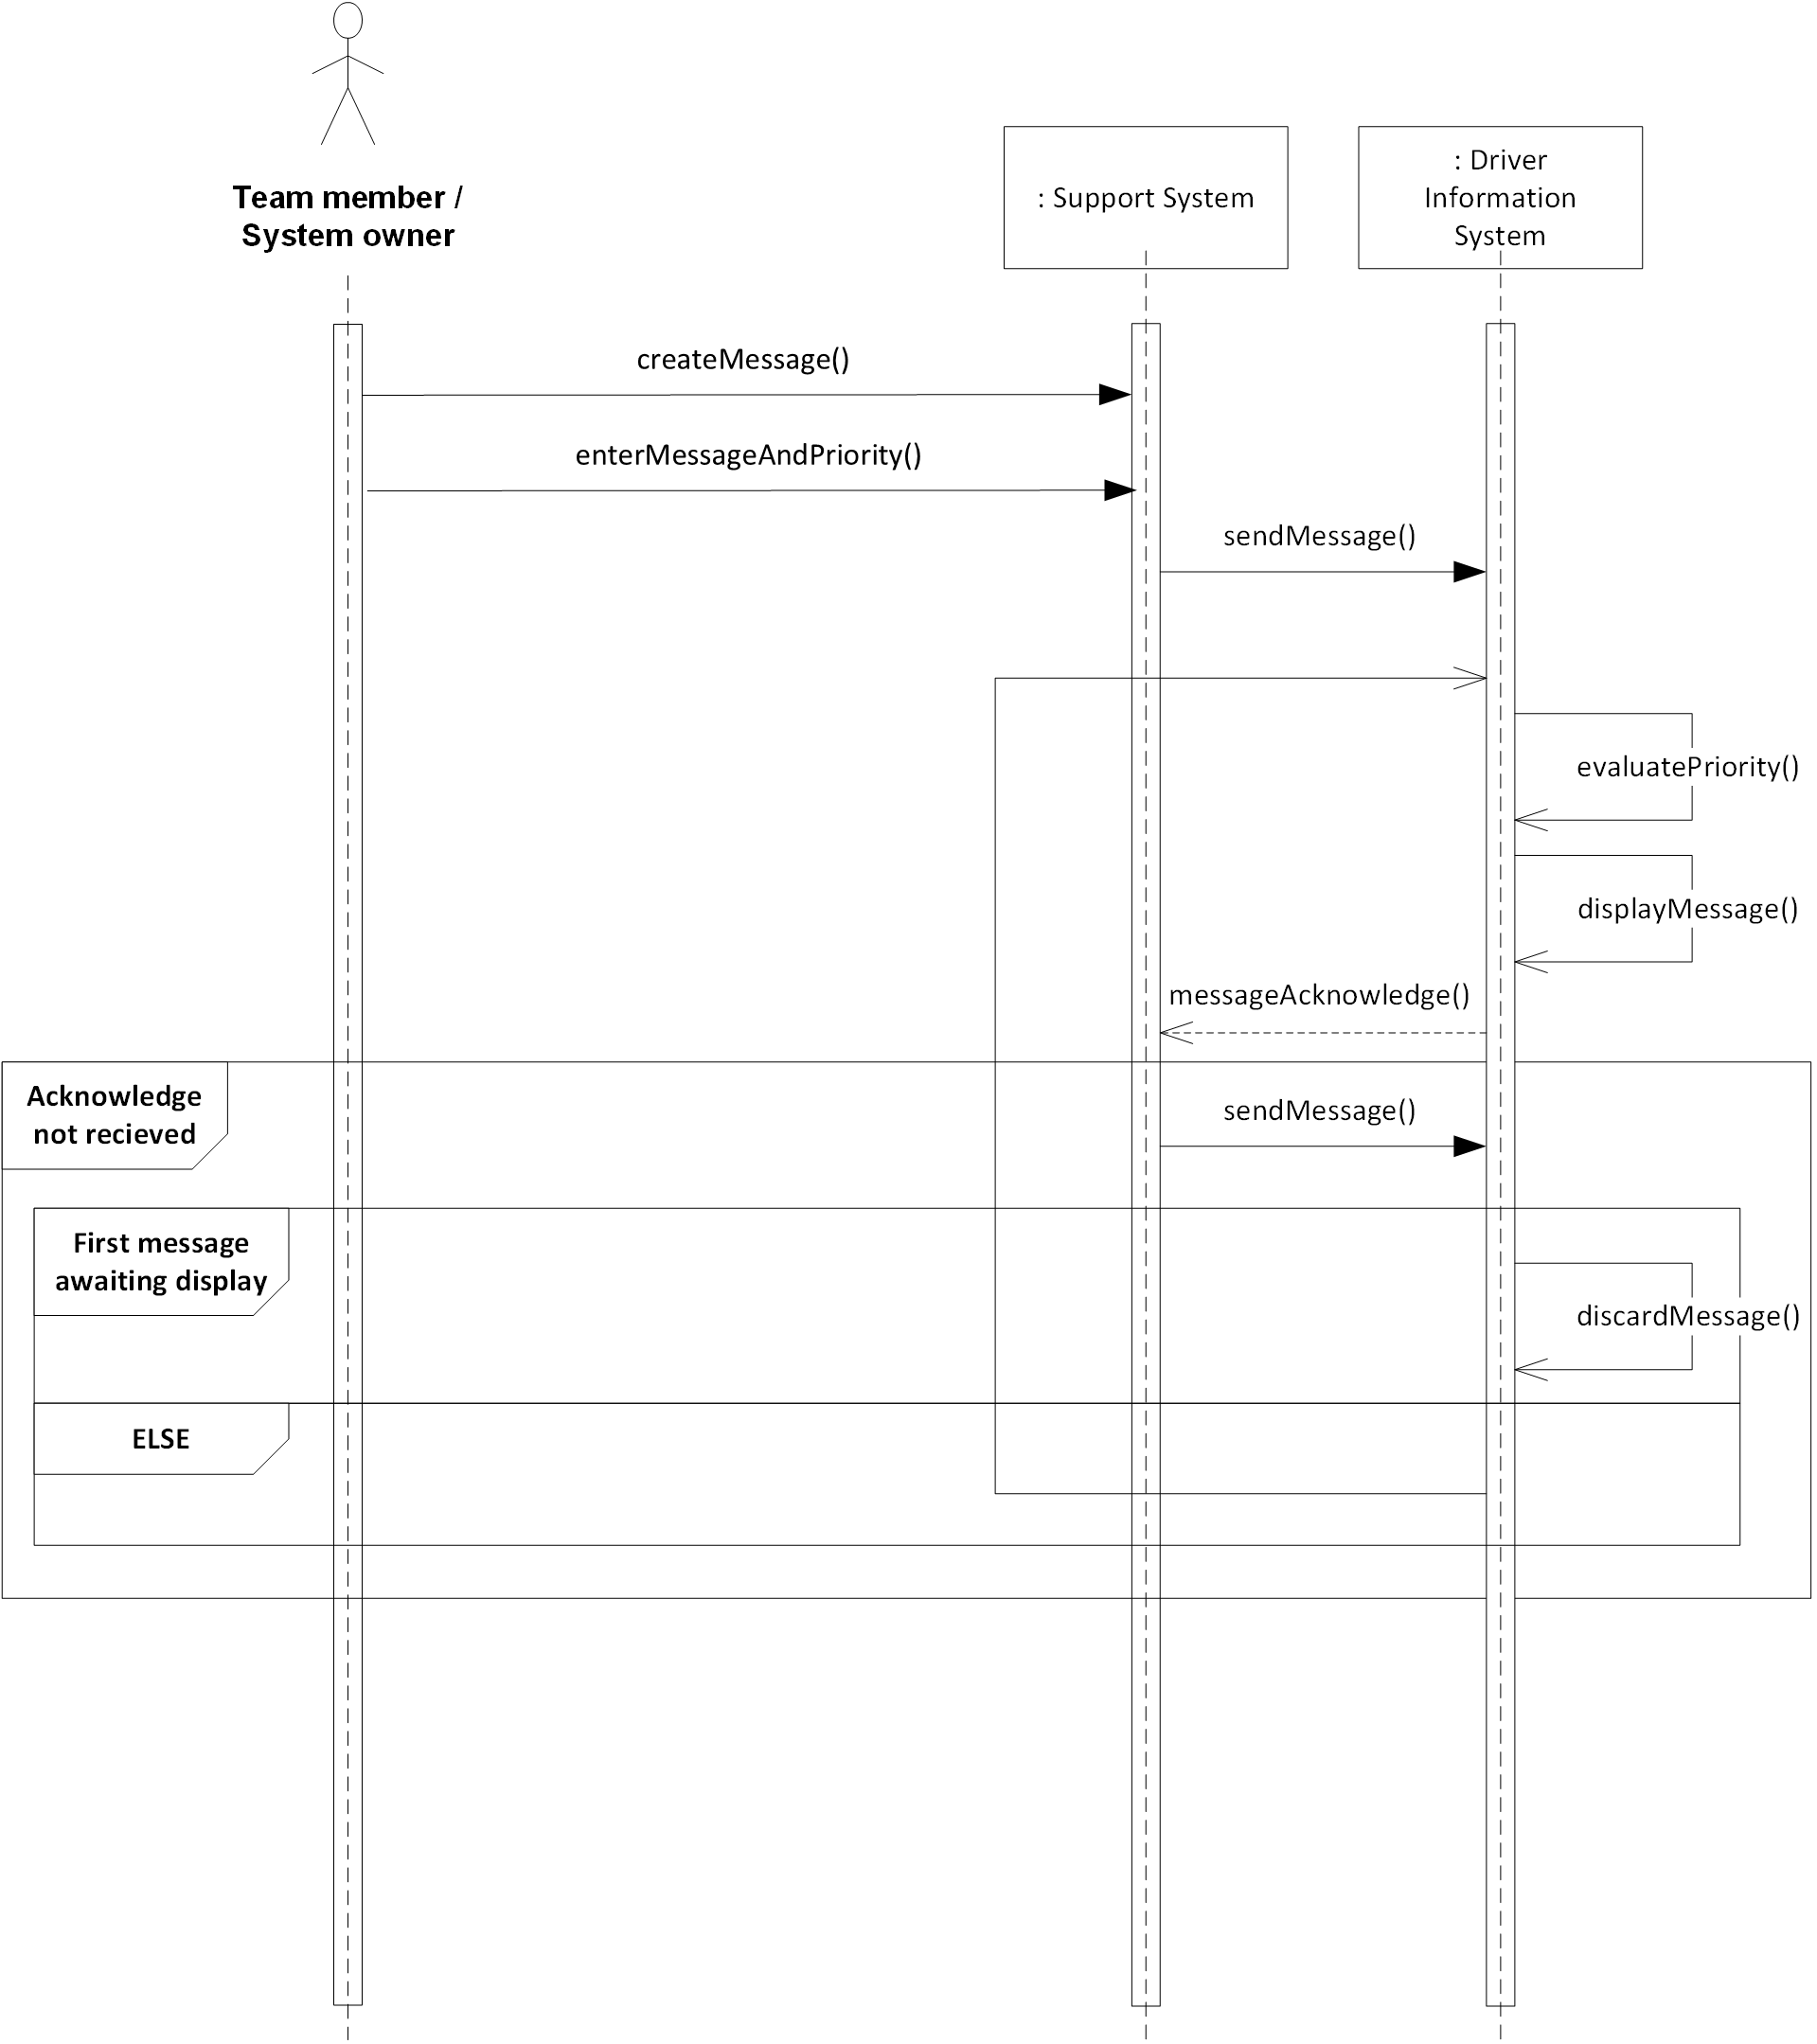
\includegraphics[width=\textwidth]{SSD-Send-Message.png}
  \caption{SSD for UC\vref{uc_dispconf}}
  \label{fig:SSD-Send-Message}
\end{figure}
\clearpage 


\subsubsection{SSD - Display Real Time Info}
\begin{figure}[!htbp]
  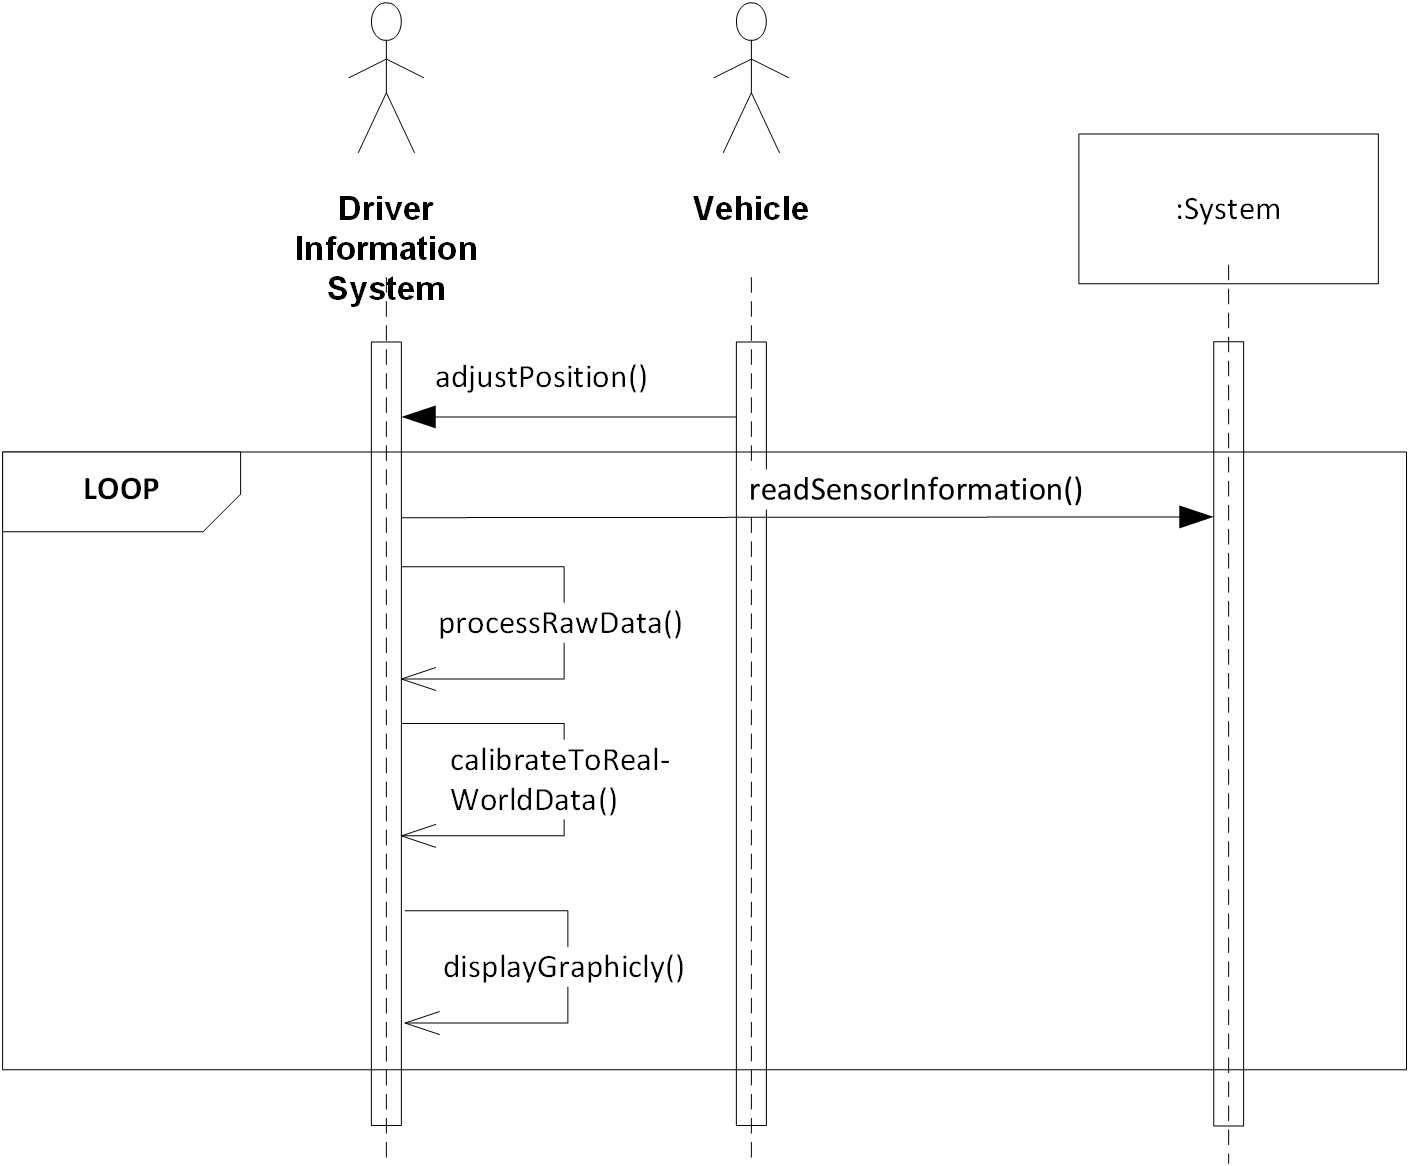
\includegraphics[width=\textwidth]{SSD-Display-Real-Time-Info.png}
  \caption{SSD for UC\vref{uc_dispconf}}
  \label{fig:SSD-Display-Real-Time-Info}
\end{figure}
\clearpage 
